%!TEX root = ../Thesis.tex
\section*{Anhang}
\addcontentsline{toc}{section}{Anhang}
\fancyhead[R]{Anhang}

\anhangsverzeichnis

\anhang{Weitere Use-Cases}\label{Anhang-Use-Cases}

\subanhang{Administrator}\label{Anhang-Admin}
\begin{figure}[h]
\centering
\begin{minipage}[t]{1\textwidth} 
\caption{Administrator Use-Case Diagramm} 
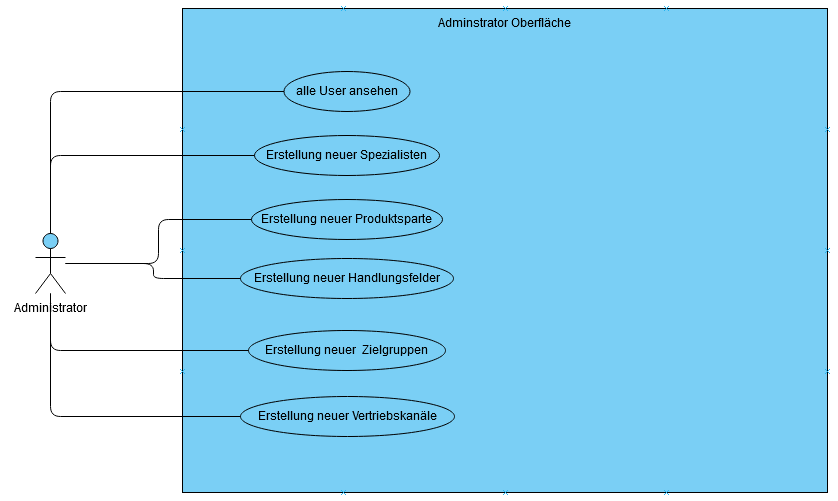
\includegraphics[width=1\textwidth]{img/admin-use-case.png}\\
\source{Eigene Darstellung} 
\end{minipage}
\end{figure}

\subanhang{Kontaktformular}\label{Anhang-Kontakt}
\begin{figure}[h]
\centering
\begin{minipage}[t]{1\textwidth} 
\caption{Kontaktformular Use-Case Diagramm} 
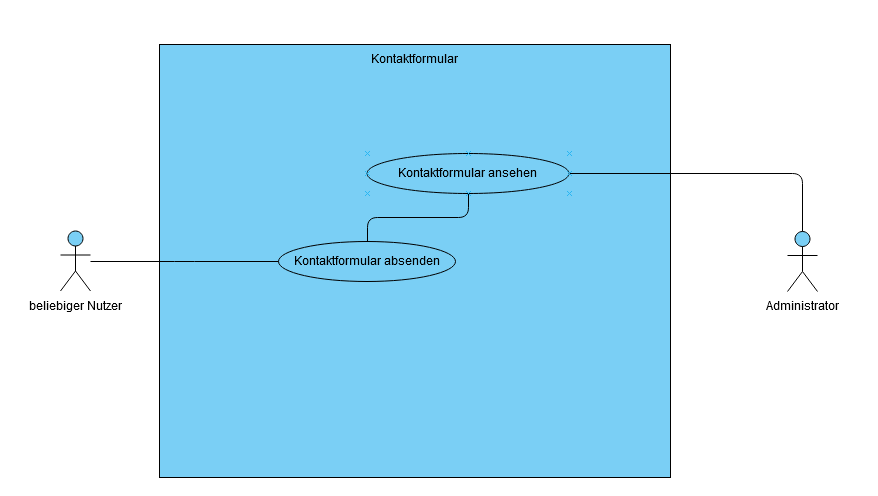
\includegraphics[width=1\textwidth]{img/kontakt-use-case.png}\\
\source{Eigene Darstellung} 
\end{minipage}
\end{figure}

\clearpage
\pagebreak

\anhang{GUI-Konzept}

\subanhang{Konzept}\label{GUI-Konzept}

\begin{figure}[h]
\centering
\begin{minipage}[t]{1\textwidth} 
\caption{GUI-Konzept - Registrierung } 
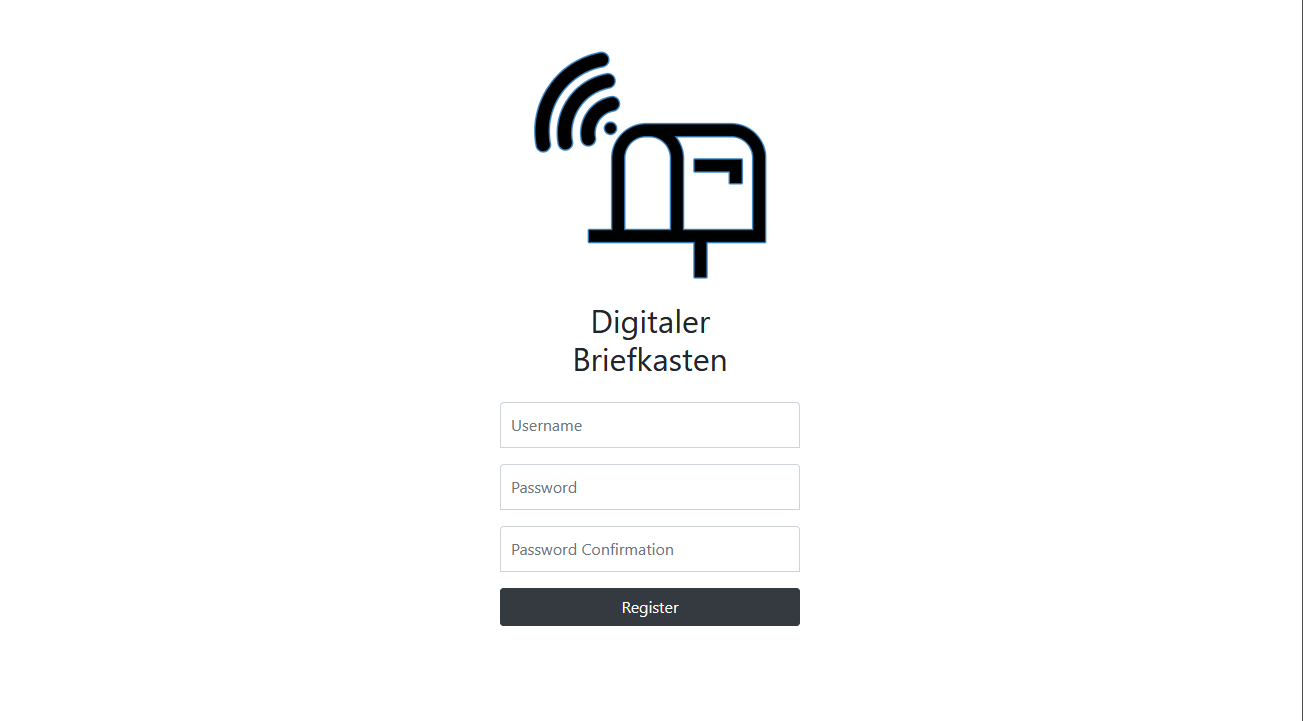
\includegraphics[width=1\textwidth]{img/registrierung-konzept.png}\\
\source{Eigene Darstellung} 
\end{minipage}
\end{figure}

\begin{figure}[h]
\centering
\begin{minipage}[t]{1\textwidth} 
\caption{GUI-Konzept - Willkommen} 
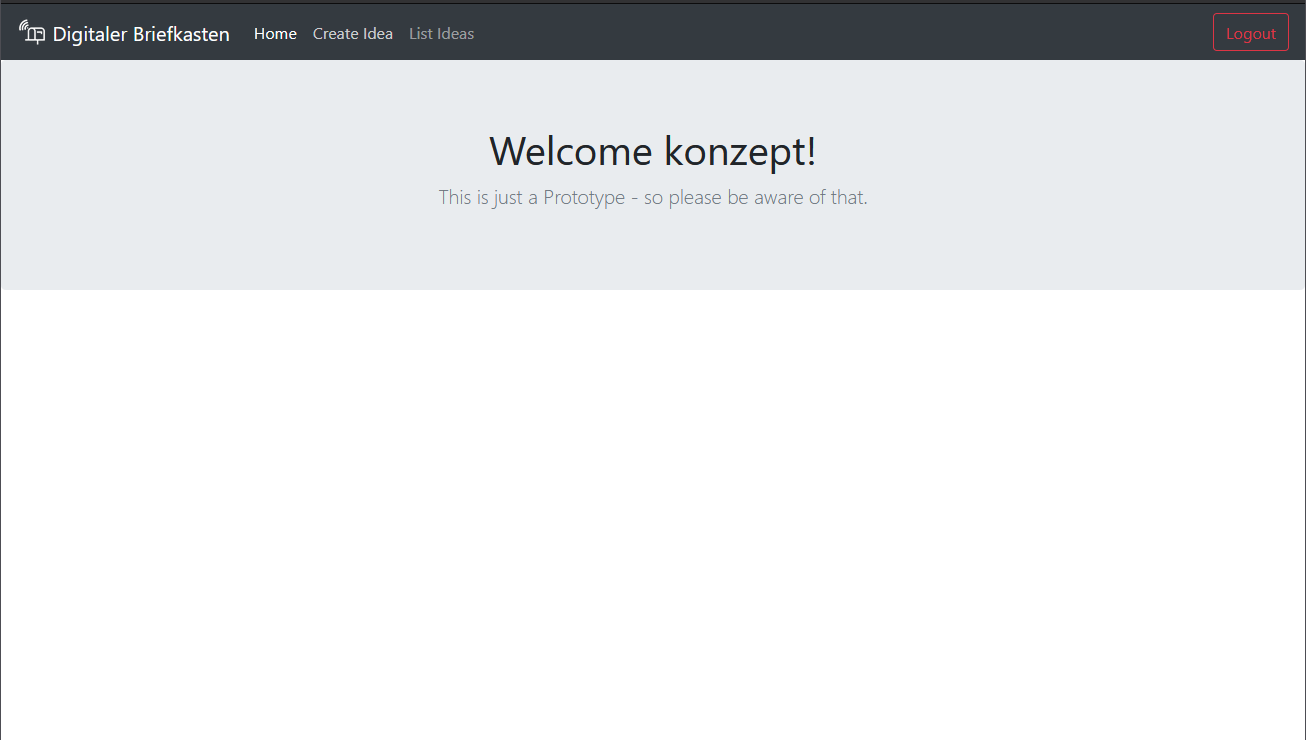
\includegraphics[width=1\textwidth]{img/welcome-konzept.png}\\
\source{Eigene Darstellung} 
\end{minipage}
\end{figure}

\begin{figure}[h]
\centering
\begin{minipage}[t]{1\textwidth} 
\caption{GUI-Konzept - Idee erstellen } 
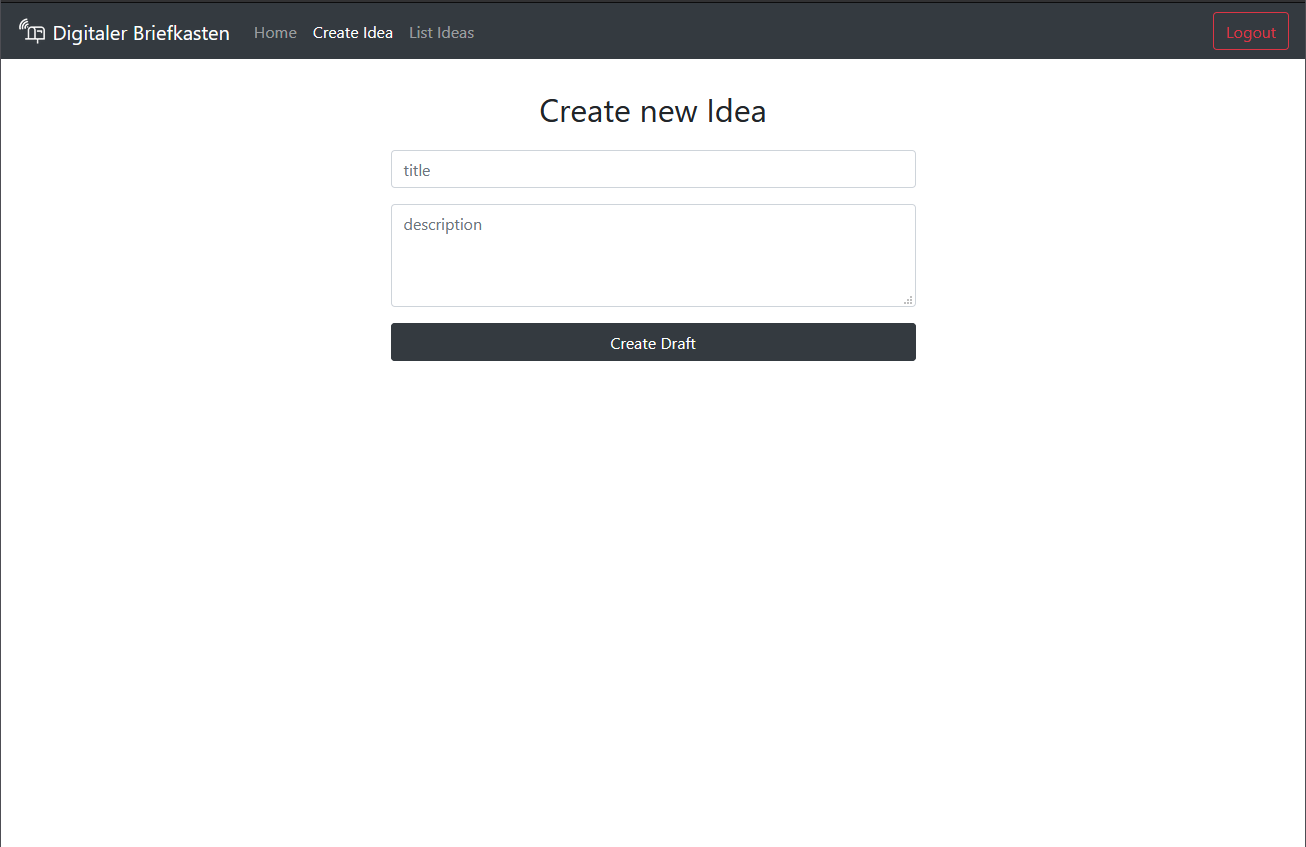
\includegraphics[width=1\textwidth]{img/createIdea-konzept.png}\\
\source{Eigene Darstellung} 
\end{minipage}
\end{figure}

\clearpage
\pagebreak

\subanhang{Umsetzung}\label{GUI-Umsetzung}

Die im folgenden dargestellten GUI Bestandteile stellen die wichtigsten Teile der Oberfläche dar. Auf die Abbildung aller Bestandteile wurde aufgrund der zu großen Menge, zur Wahrung der Übersichtlichkeit, verzichtet.

\begin{figure}[h]
\centering
\begin{minipage}[t]{1\textwidth} 
\caption{GUI-Umsetzung - Login } 
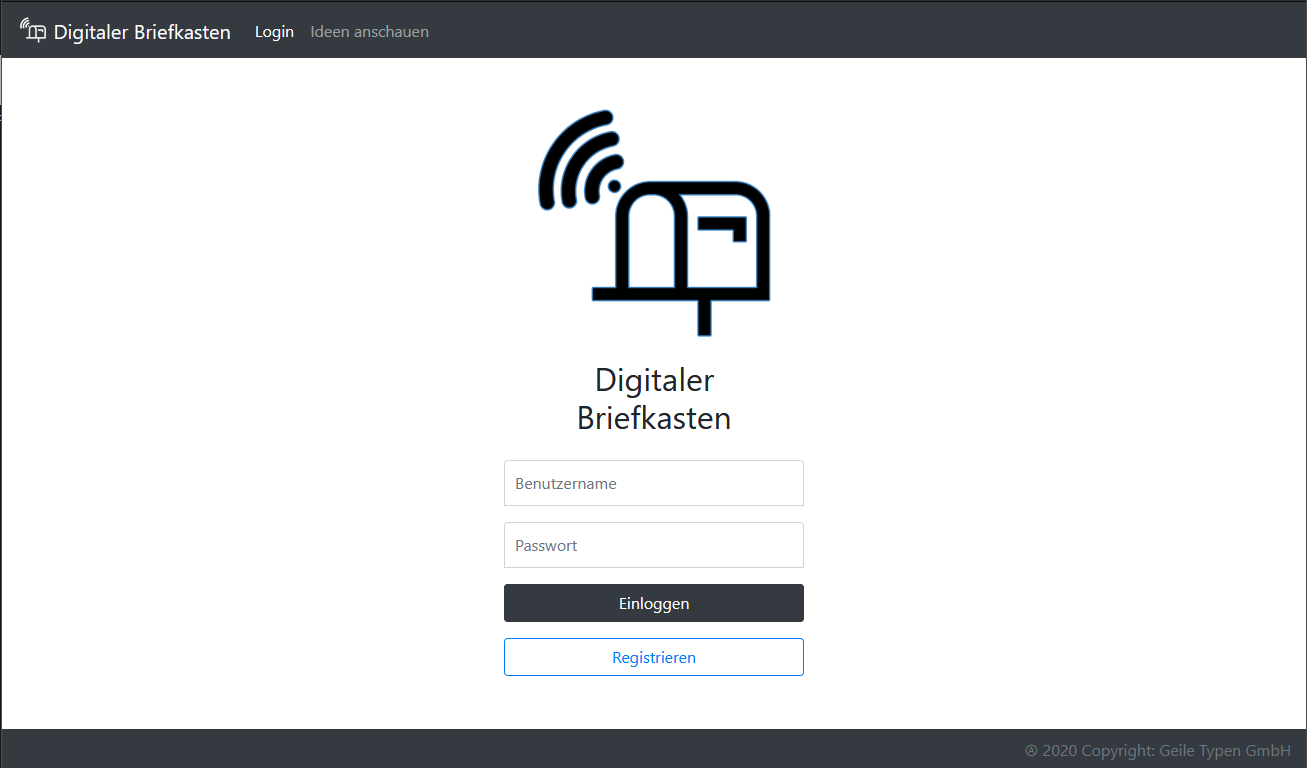
\includegraphics[width=1\textwidth]{img/login-umsetzung.png}\\
\source{Eigene Darstellung} 
\end{minipage}
\end{figure}

\begin{figure}[h]
\centering
\begin{minipage}[t]{1\textwidth} 
\caption{GUI-Umsetzung - Registrierung } 
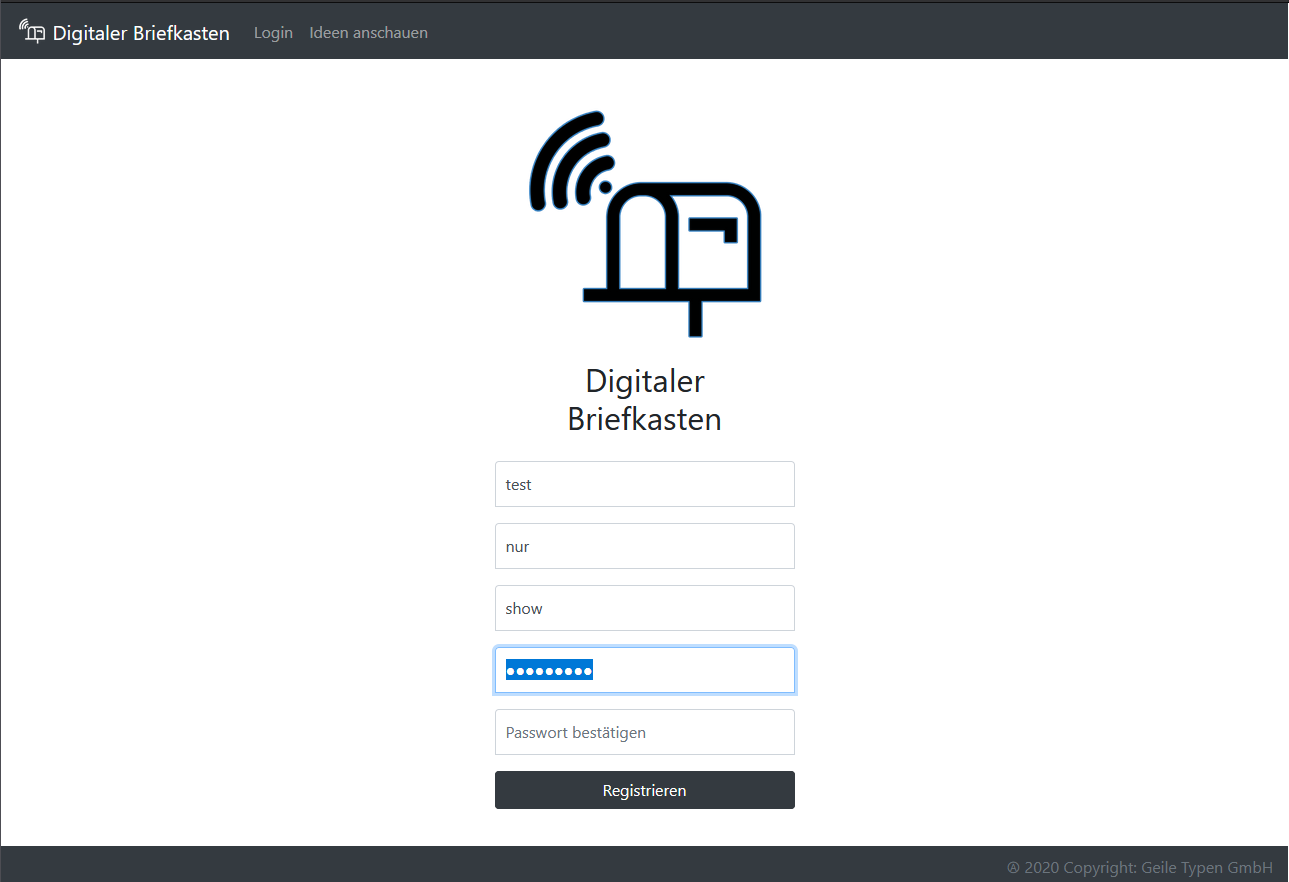
\includegraphics[width=1\textwidth]{img/registrierung-umsetzung.png}\\
\source{Eigene Darstellung} 
\end{minipage}
\end{figure}

\begin{figure}[h]
\centering
\begin{minipage}[t]{1\textwidth} 
\caption{GUI-Umsetzung - Ideen}
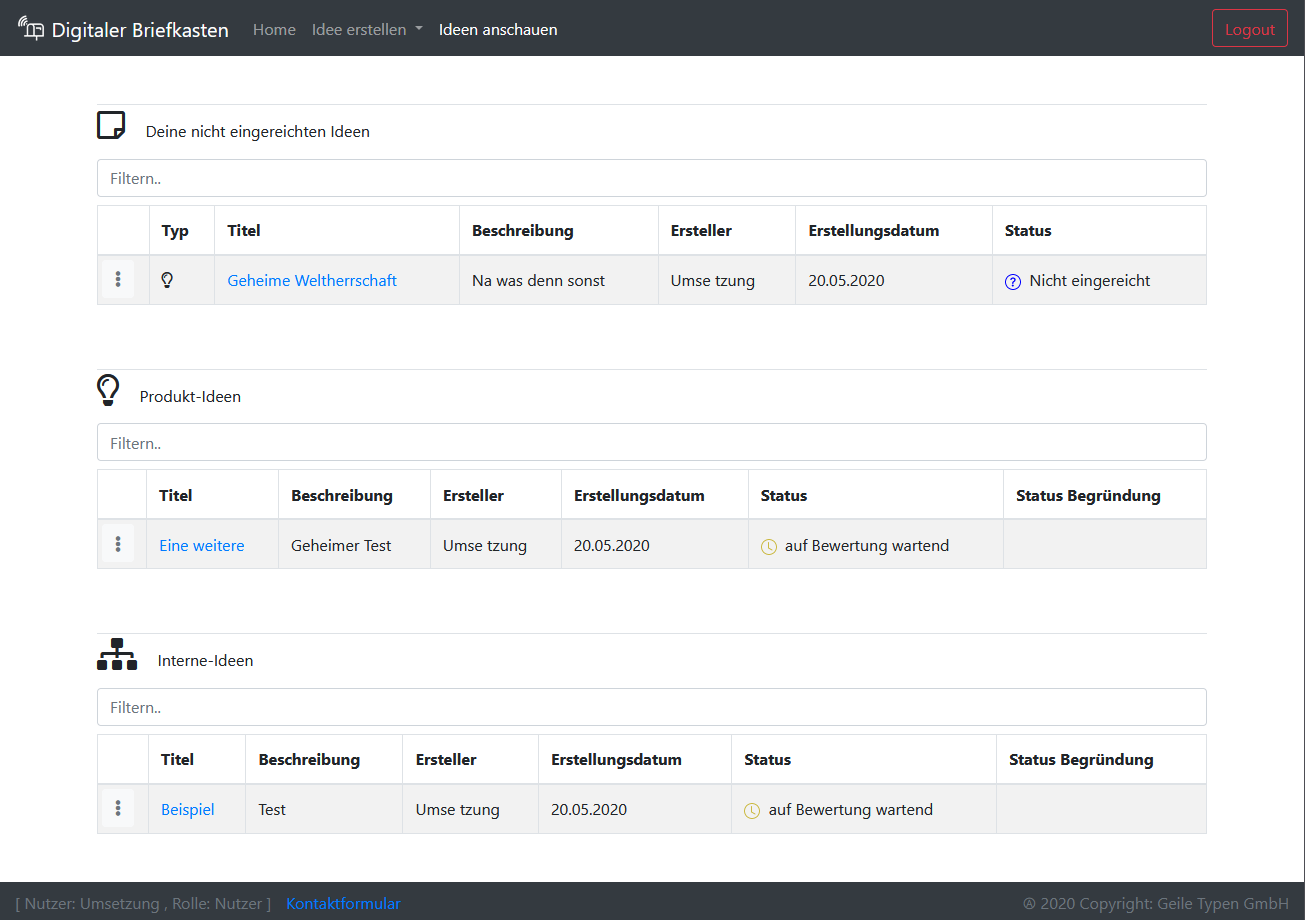
\includegraphics[width=1\textwidth]{img/ideen-umsetzung.png}\\
\source{Eigene Darstellung} 
\end{minipage}
\end{figure}

\begin{figure}[h]
\centering
\begin{minipage}[t]{1\textwidth} 
\caption{GUI-Umsetzung - Idee erstellen } 
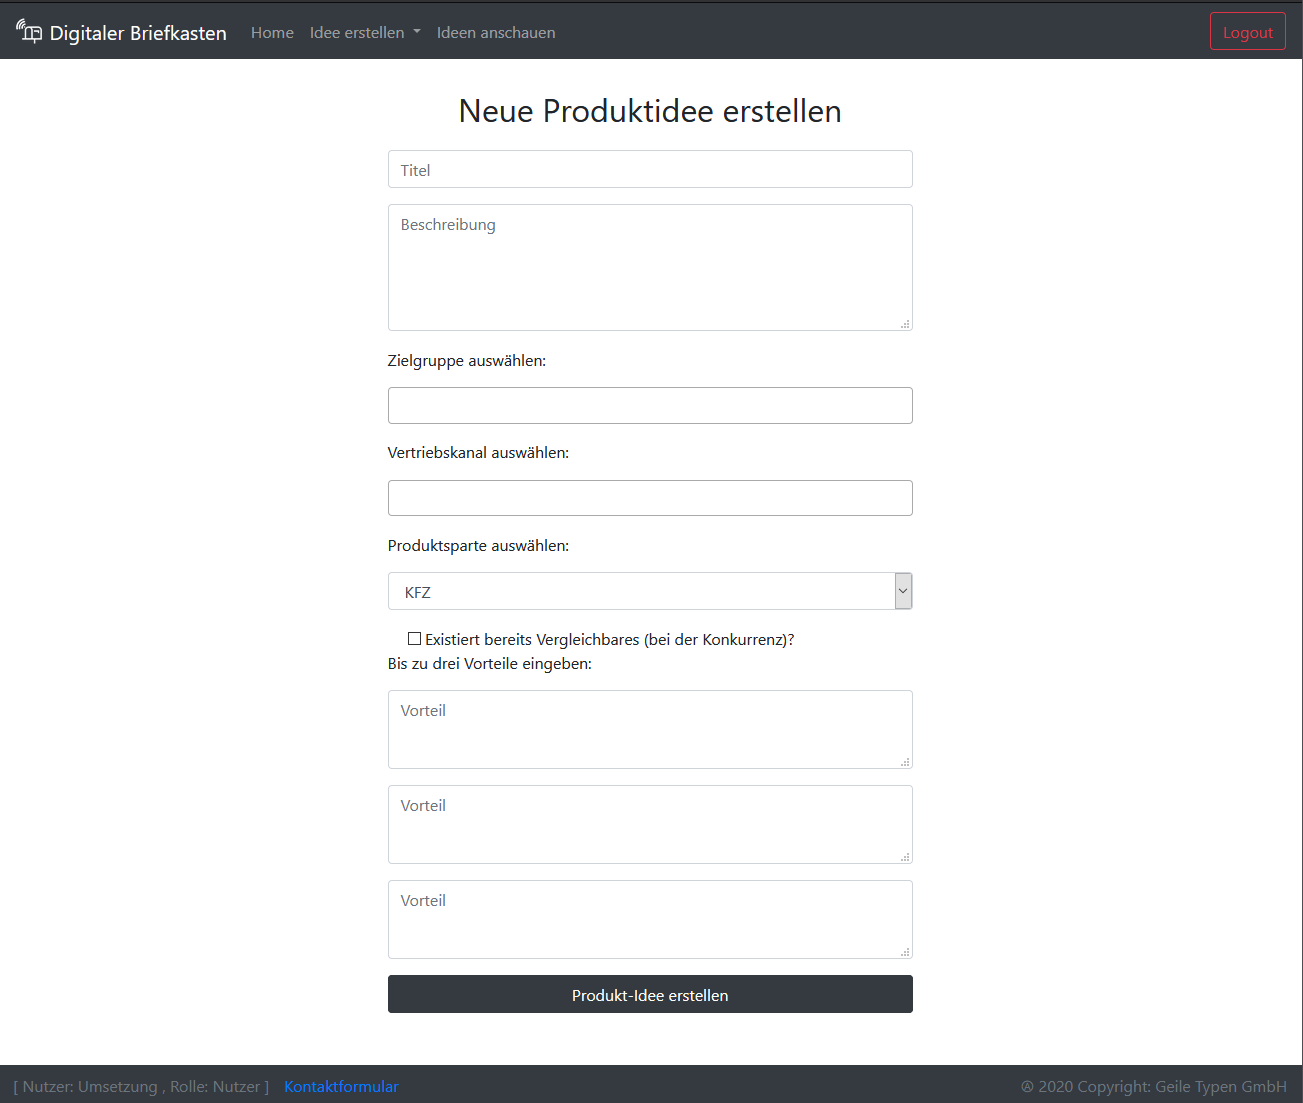
\includegraphics[width=1\textwidth]{img/createIdea-umsetzung.png}\\
\source{Eigene Darstellung} 
\end{minipage}
\end{figure}

\begin{figure}[h]
\centering
\begin{minipage}[t]{1\textwidth} 
\caption{GUI-Umsetzung - Idee ansehen } 
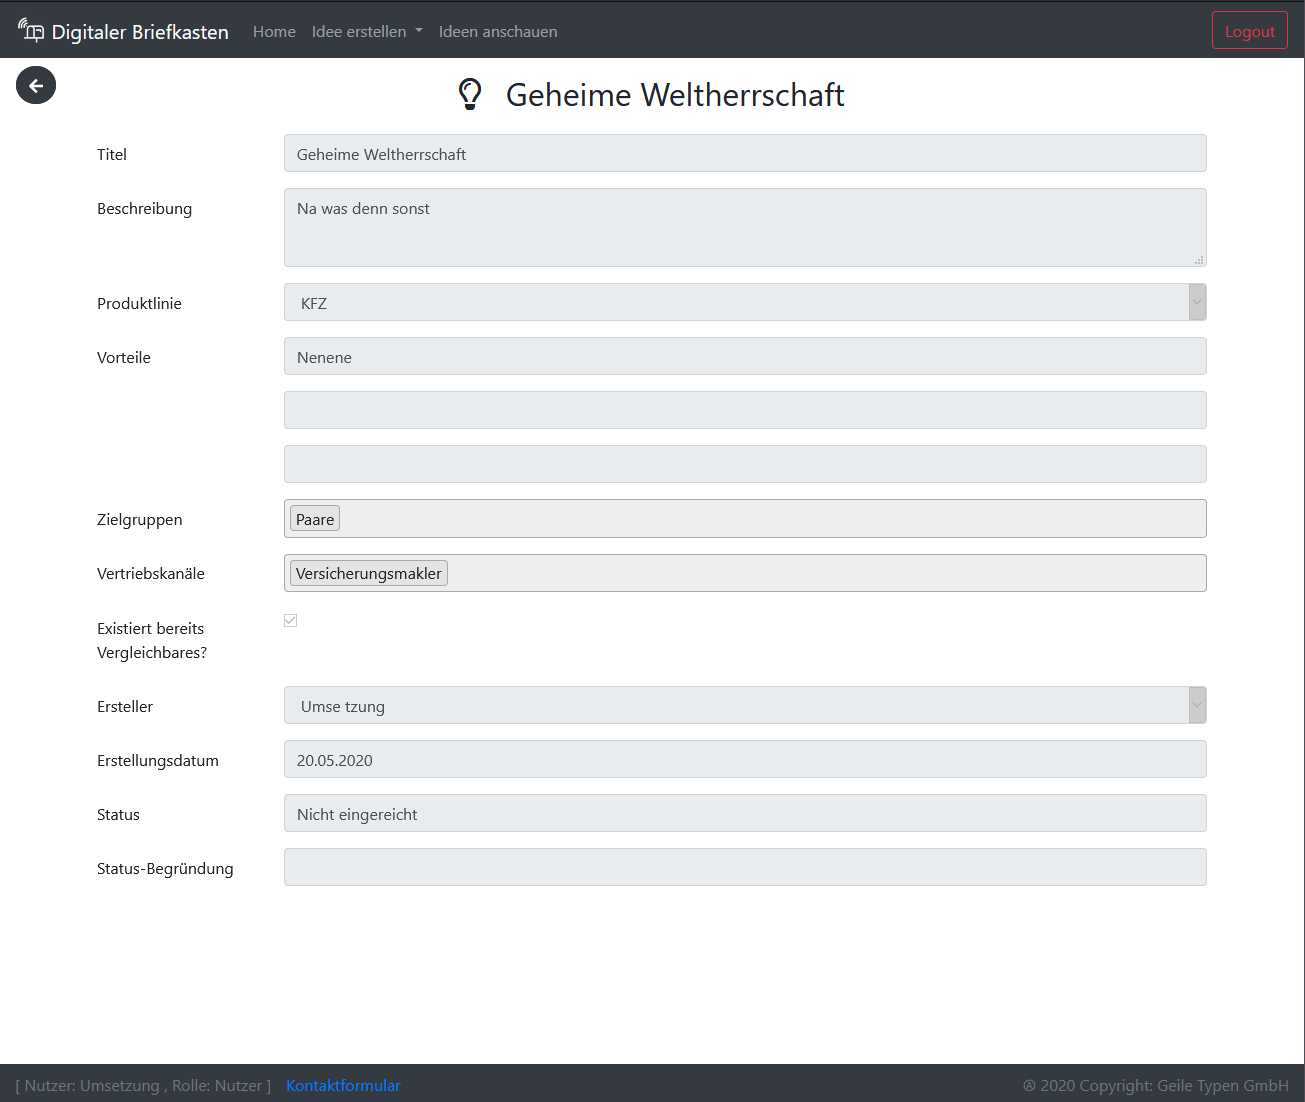
\includegraphics[width=1\textwidth]{img/idee-umsetzung.png}\\
\source{Eigene Darstellung} 
\end{minipage}
\end{figure}

\begin{figure}[h]
\centering
\begin{minipage}[t]{1\textwidth} 
\caption{GUI-Umsetzung - Admin Ansicht } 
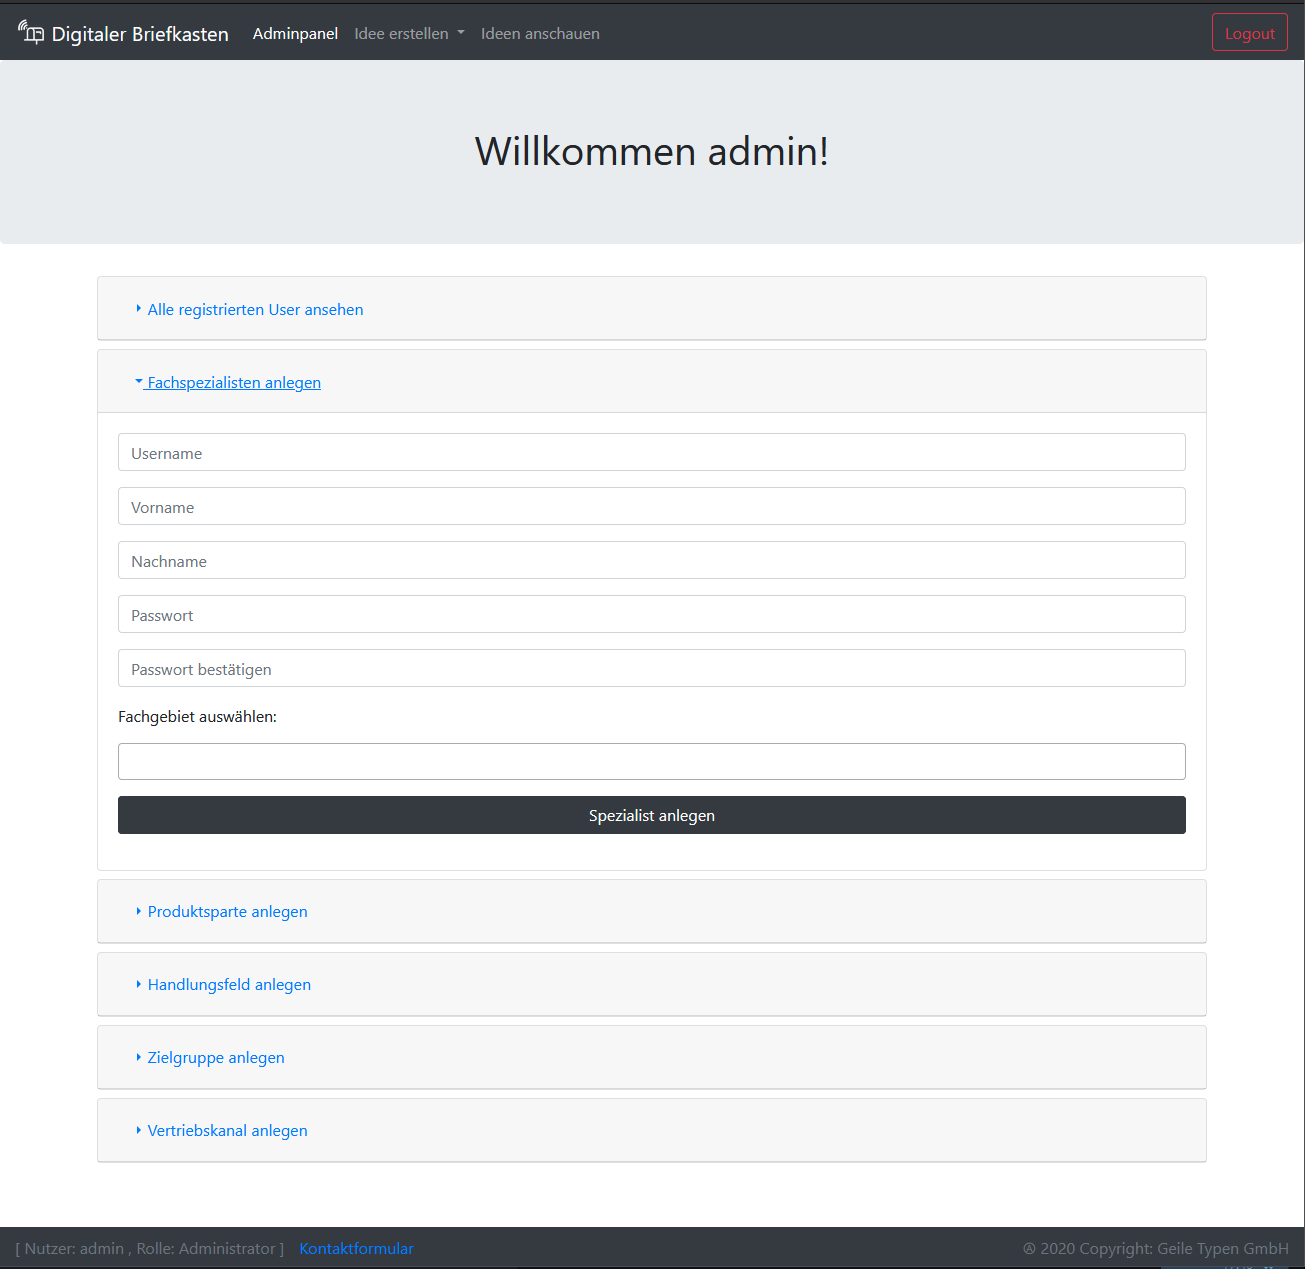
\includegraphics[width=1\textwidth]{img/admin-umsetzung.png}\\
\source{Eigene Darstellung} 
\end{minipage}
\end{figure}

\begin{figure}[h]
\centering
\begin{minipage}[t]{1\textwidth} 
\caption{GUI-Umsetzung - Spezialist Ansicht } 
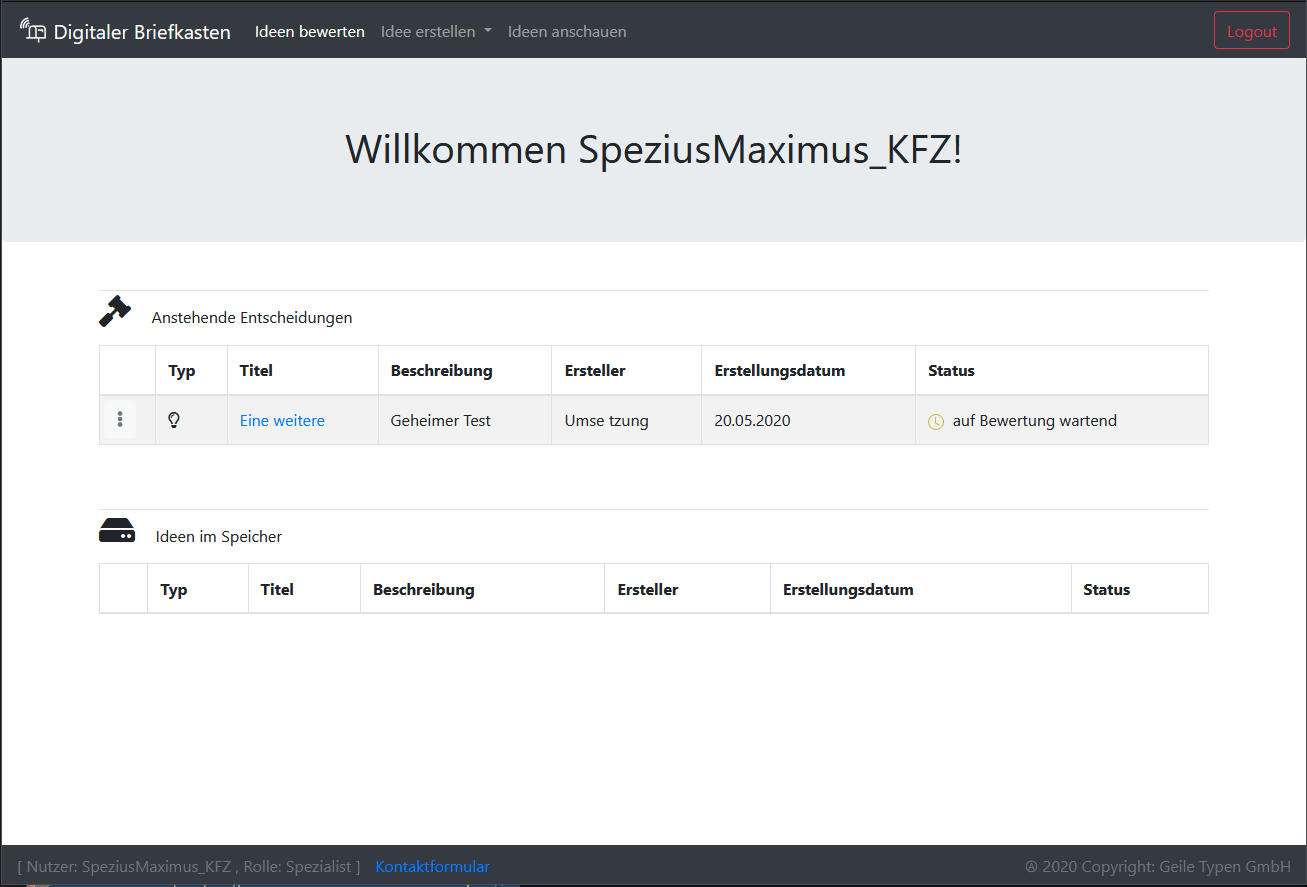
\includegraphics[width=1\textwidth]{img/spezialist-umsetzung.png}\\
\source{Eigene Darstellung} 
\end{minipage}
\end{figure}
